% !TeX root = ../main.tex
% Add the above to each chapter to make compiling the PDF easier in some editors.

\chapter{Theory}\label{chapter:theory}

In this chapter, we introduce the theoretical foundations for our subsequent work. We begin by formally introducing the metrics we use to assess the performance of the discussed algorithms. We then introduce the problem of smoothed convex optimization and related variants that the examined algorithms address.

\section{Performance Metrics}\label{section:theory:performance_metrics}

We say that an algorithm is \emph{optimal}\index{optimal algorithm} with respect to some performance metric if no algorithm can achieve a better score in the given metric given the same information. Crucially, optimality depends on the information given to the algorithm. We thus say that an offline algorithm of a minimization problem is optimal if its result always incurs the smallest possible cost while satisfying the given constraints. In contrast, an optimal online algorithm must not necessarily return the optimal offline solution. In fact, in many cases, online algorithms must necessarily perform worse than optimal offline algorithms due to the lack of provided information (in our case, the convex cost functions arrive over time). Naturally, these performance metrics also inform parts of our experimental analysis performed in \cref{chapter:case_studies}.

\subsection{Approximations}

We begin by considering the offline case. In most cases, we seek to find optimal solutions to the offline problem. However, for some problems where the computational complexity of optimal solutions is high for large instances, it is beneficial to consider efficient algorithms that achieve close to optimal performance, motivating the definition of approximation algorithms. Note that we limit our definitions of performance metrics to minimization problems.

\begin{definition}\index{approximation ratio}
\cite{Williamson2011} An $\alpha$-approximation algorithm for a minimization problem $c$ is a polynomial-time algorithm $ALG$ that for all instances of the problem produces a solution whose value is within a factor of $\alpha$ of the value of an optimal solution $OPT$, i.e., $c(ALG) \leq \alpha \cdot c(OPT)$.
\end{definition}

In other words, an $\alpha$-approximation guarantees that its results are at most a factor of $\alpha$ worse than the optimal solution. The integral smoothed convex optimization problem is an example where \citeauthor*{Kappelmann2017}~\cite{Kappelmann2017} and \citeauthor*{Albers2021_2}~\cite{Albers2021_2} recently made substantial progress on approximation algorithms.

\subsection{Competitiveness}

For online algorithms, it is natural to consider an adaptation of the idea of approximation algorithms. Here, we compare the result of an online algorithm with the optimal offline solution.

\begin{definition}\index{competitive ratio}
An $\alpha$-competitive online algorithm for a minimization problem $c$ is an algorithm $ALG$ that for all instances of the problem produces a solution whose value is within a factor of $\alpha$ of the value of an optimal offline solution $OPT$, i.e. $c(ALG) \leq \alpha \cdot c(OPT)$.
\end{definition}

We observe that this definition is analogous to our earlier definition of approximation algorithms in the offline case. However, in contrast to approximation algorithms, where the limiting factor was the algorithm's complexity, the competitiveness of online algorithms is fundamentally restricted by the information available to an online algorithm compared to its offline variants. In smoothed convex optimization, considerable work has focused on finding online algorithms with a constant competitive ratio in the number of dimensions $d$.

Crucially, the competitiveness of an online algorithm depends on the assumed adversary model. Commonly, three adversary models are used in the literature, which are described by \citeauthor*{Borodin1990}~\cite{Borodin1990}. First, the \emph{oblivious adversary}\index{oblivious adversary} is the weakest adversary and only knows the algorithm's code but needs to construct the request sequence before any moves are made. Second, the \emph{adaptive online adversary}\index{adaptive online adversary} makes the next request based on the algorithm's previous answers but serves it immediately. Third, the \emph{adaptive offline adversary}\index{adaptive offline adversary} is the strongest adversary that serves the requests based on the algorithm's previous answers but, in the end, can choose the optimal request sequence among all possible request sequences. Note that as all adversaries know the algorithm's code, they are equivalent in the case of a deterministic algorithm. Also, note that randomization is not helpful when playing against an adaptive offline adversary. In the case of many smoothed online convex optimization problems, including right-sizing data centers, it is reasonable to assume an oblivious adversary as typically incoming requests arrive independently from previous server configurations in a data center.

\subsection{Regret}

Regret is another approach to measuring the performance of online algorithms.

\begin{definition}\index{regret (static)}
The (static) regret of an online algorithm $ALG$ for a minimization problem $c$ is $\rho(T)$ if for all instances of the problem the difference between the result of the algorithm and the static optimal offline solution $OPT_s$ does not exceed $\rho(T)$, i.e. $c(ALG) - c(OPT_s) \leq \rho(T)$.
\end{definition}

Commonly, the literature considers this definition of regret where the online algorithm is compared against a static offline solution, i.e., a solution where the agent is not allowed to move in the decision space. We say that an algorithm achieves \emph{no-regret}\index{no-regret} if $\rho$ is sublinear in the time horizon $T$. Observe that ideally, an algorithm achieves negative regret, in which case it performs better than the static optimum.

Ideally, online algorithms perform well with respect to the competitive ratio and regret. In other words, our online algorithms should both perform well compared against an agent that is moving in the decision space with perfect knowledge of the future (competitive ratio) and perform well against an agent that picks one optimal location in the decision space. In practice, for the example of dynamically right-sizing a data center, our algorithms are required to outperform a static number of servers to be viable alternatives. In contrast, to minimize energy waste and revenue loss, the strategies proposed by our algorithms must be as close as possible to the optimal dynamic strategies.

However, \citeauthor*{Andrew2015}~\cite{Andrew2015} proved that no online algorithm for smoothed convex optimization can simultaneously achieve a constant competitive ratio and no-regret even when $d = 1$ and cost functions are linear. The competitive ratio can be arbitrarily poor for no-regret algorithms by oscillating the dynamic optimal solution between two points in the decision space. The no-regret algorithm will approach a static optimum, which can be arbitrarily worse than the dynamic optimum. In contrast, a constant-competitive algorithm generally sticks to a point in the decision space until it knows that the cost of movement is outweighed by the reduced cost of some other point that it then moves to. Hence, for constant-competitive algorithms, the regret can be arbitrarily large as the algorithm oscillates between the two points in the decision space, in each step having an arbitrary distance to the static optimum. An illustrative example with one dimension and a periodic sequence of two linear cost functions is depicted in \cref{fig:incompatibility_of_competitive_ratio_and_regret}.

\begin{figure}
    \centering
    


\tikzset{every picture/.style={line width=0.75pt}} %set default line width to 0.75pt

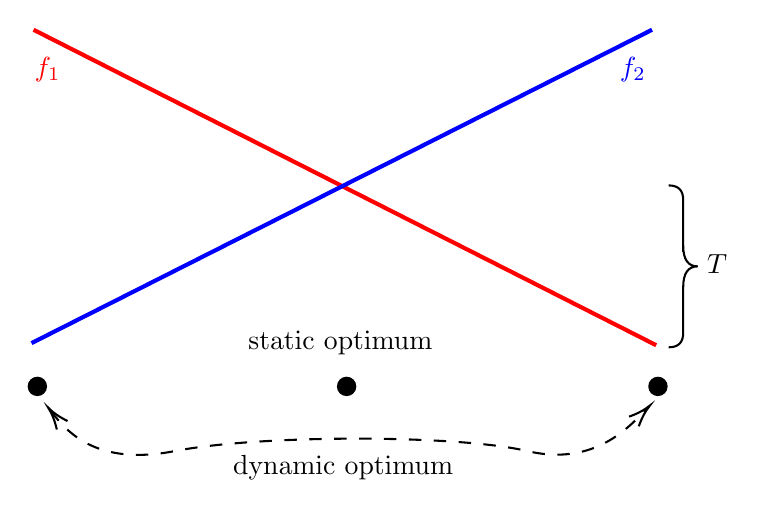
\begin{tikzpicture}[x=0.75pt,y=0.75pt,yscale=-1,xscale=1]
%uncomment if require: \path (0,300); %set diagram left start at 0, and has height of 300

%Shape: Circle [id:dp3024076819219861]
\draw  [fill=black  ,fill opacity=1 ] (305.67,223.17) .. controls (305.67,220.87) and (307.53,219) .. (309.83,219) .. controls (312.13,219) and (314,220.87) .. (314,223.17) .. controls (314,225.47) and (312.13,227.33) .. (309.83,227.33) .. controls (307.53,227.33) and (305.67,225.47) .. (305.67,223.17) -- cycle ;
%Shape: Circle [id:dp7041225921361765]
\draw  [fill=black  ,fill opacity=1 ] (156.67,223.17) .. controls (156.67,220.87) and (158.53,219) .. (160.83,219) .. controls (163.13,219) and (165,220.87) .. (165,223.17) .. controls (165,225.47) and (163.13,227.33) .. (160.83,227.33) .. controls (158.53,227.33) and (156.67,225.47) .. (156.67,223.17) -- cycle ;
%Shape: Circle [id:dp8996341089567816]
\draw  [fill=black  ,fill opacity=1 ] (455.67,223.17) .. controls (455.67,220.87) and (457.53,219) .. (459.83,219) .. controls (462.13,219) and (464,220.87) .. (464,223.17) .. controls (464,225.47) and (462.13,227.33) .. (459.83,227.33) .. controls (457.53,227.33) and (455.67,225.47) .. (455.67,223.17) -- cycle ;
%Curve Lines [id:da9487169876590669]
\draw [line width=0.75]  [dash pattern={on 4.5pt off 4.5pt}]  (167.3,235) .. controls (174.51,244.28) and (188.46,261.85) .. (227,254.33) .. controls (268,246.33) and (363,246.33) .. (397,254.33) .. controls (429.3,261.93) and (446.27,242.44) .. (454.73,233.63) ;
\draw [shift={(456,232.33)}, rotate = 495] [color=black  ][line width=0.75]    (10.93,-3.29) .. controls (6.95,-1.4) and (3.31,-0.3) .. (0,0) .. controls (3.31,0.3) and (6.95,1.4) .. (10.93,3.29)   ;
\draw [shift={(166,233.33)}, rotate = 51.55] [color=black  ][line width=0.75]    (10.93,-3.29) .. controls (6.95,-1.4) and (3.31,-0.3) .. (0,0) .. controls (3.31,0.3) and (6.95,1.4) .. (10.93,3.29)   ;
%Straight Lines [id:da002446124086751267]
\draw [color=red  ,draw opacity=1 ][line width=1.5]    (159,51.33) -- (459,203.33) ;
%Straight Lines [id:da715905705967314]
\draw [color=blue  ,draw opacity=1 ][line width=1.5]    (158,202.33) -- (457,51.33) ;
%Shape: Brace [id:dp3550286018056783]
\draw  [line width=0.75]  (465,204.33) .. controls (469.67,204.33) and (472,202) .. (472,197.33) -- (472,175.33) .. controls (472,168.66) and (474.33,165.33) .. (479,165.33) .. controls (474.33,165.33) and (472,162) .. (472,155.33)(472,158.33) -- (472,133.33) .. controls (472,128.66) and (469.67,126.33) .. (465,126.33) ;

% Text Node
\draw (240,255) node [anchor=north west][inner sep=0.75pt]   [align=left] {\begin{minipage}[lt]{100pt}\setlength\topsep{0pt}
\begin{center}
dynamic optimum
\end{center}

\end{minipage}};
% Text Node
\draw (252,195) node [anchor=north west][inner sep=0.75pt]   [align=left] {\begin{minipage}[lt]{80pt}\setlength\topsep{0pt}
\begin{center}
static optimum
\end{center}

\end{minipage}};
% Text Node
\draw (158,63) node [anchor=north west][inner sep=0.75pt]  [color=red  ,opacity=1 ]  {$f_{1}$};
% Text Node
\draw (440,63) node [anchor=north west][inner sep=0.75pt]  [color=blue  ,opacity=1 ]  {$f_{2}$};
% Text Node
\draw (482,158) node [anchor=north west][inner sep=0.75pt]    {$T$};


\end{tikzpicture}

    \caption{Incompatibility of competitive ratio and regret in one dimension. Consider an adversary playing two linear cost functions $f_1$ and $f_2$ with different minimizers. Then, the dynamic optimum oscillates between the two minimizers while the the static optimum is given by the intersection of the two cost functions. Therefore, a no-regret algorithm may be arbitrarily far away from the dynamic offline optimum. In contrast, a competitive algorithm which sticks to either end of the decision space may exceed the static offline optimum by a delta that is not in $\mathcal{O}(T)$ \cite{Wierman2019}.}
    \label{fig:incompatibility_of_competitive_ratio_and_regret}
\end{figure}

There thus exist many variants of regret and the competitive ratio used to bridge between the two metrics. One approach considers an additive variant of the competitive ratio, which is called the \emph{competitive difference}.

\begin{definition}\index{competitive difference}
\cite{Chen2015} The competitive difference of an online algorithm $ALG$ for a minimization problem $c$ is $\rho(T)$ if for all instances of the problem, the difference between the result of the algorithm and the dynamic optimal offline solution $OPT$ does not exceed $\rho(T)$, i.e., $c(ALG) - c(OPT) \leq \rho(T)$.
\end{definition}

This definition is also known as \emph{dynamic regret}\index{dynamic regret}~\cite{Chen2018}. We next define a variant of regret that bridges between static and dynamic regret.

\begin{definition}\index{constrained dynamic regret}
\cite{Chen2018} The $L$-constrained dynamic regret of an online algorithm $ALG$ for a minimization problem $c$ is $\rho(T)$ if for all instances of the problem the difference between the result of the algorithm and the $L$-constrained optimal offline solution $OPT_L$ does not exceed $\rho(T)$, i.e. $c(ALG) - c(OPT_L) \leq \rho(T)$.

The $L$-constrained optimal offline solution minimizes $c$ subject to the additional constraint \begin{align*}
    \sum_{t=1}^T \norm{X_t - X_{t-1}} \leq L
\end{align*} for $X_t, X_{t-1} \in \mathcal{X}$.
\end{definition}

We now observe that given the optimal offline solution $OPT$ with schedule $\hat{X}_t$, the $L$-constrained dynamic regret is equivalent to dynamic regret for $L = \sum_{t=1}^T \norm{\hat{X}_t - \hat{X}_{t-1}}$. In contrast, given the static optimal offline solution $OPT_s$, the $L$-constrained dynamic regret is equivalent to static regret for $L = \norm{OPT_s - \mathbf{0}}$ which is the initial (and only) step of $OPT_s$~\cite{Chen2018}.

Another metric used to bridge the gap between the competitive ratio and regret is the \emph{$\alpha$-unfair competitive ratio} which penalizes movement in the decision space by an additional factor $\alpha$~\cite{Andrew2015}.

\begin{definition}\index{unfair competitive ratio}
\cite{Andrew2015} The $\alpha$-unfair competitive ratio of an online algorithm $ALG$ for a minimization problem $c$ is $\beta$ if for all instances of the problem the ratio of the result of the algorithm and the dynamic $\alpha$-unfair offline solution $OPT_{\alpha}$ does not exceed $\beta$, i.e. $c(ALG) \leq \beta \cdot c(OPT_{\alpha})$.

Here, the $\alpha$-unfair optimal offline solution $OPT_{\alpha}$ is defined as the minimizer of \begin{align*}
    \sum_{t=1}^T f_t(X_t) + \alpha \norm{X_t - X_{t-1}}.
\end{align*}
\end{definition}

Note that for $\alpha = 1$, the $\alpha$-unfair competitive ratio is equivalent to the competitive ratio. For large $\alpha$, the $\alpha$-unfair optimal offline solution $OPT_{\alpha}$ is similar to the $L$-constrained optimal offline solution $OPT_L$ in that the movement in the decision space is restricted.

\section{Problems}

Now that we have an overview of the commonly used performance metrics, we introduce the problems we consider in this work. We initially state the problems as offline problems, but as all problems follow the same structure, their corresponding online variant is obtained by deferring the convex cost functions. All other problem variables --- except for the time horizon $T$ --- such as the movement cost that penalizes movement in the decision space are known from the beginning.

\subsection{Smoothed Convex Optimization}

We begin by formally introducing the most general problem we consider and which we already motivated in \cref{chapter:introduction}.

\begin{problem}[Smoothed Convex Optimization (SCO)]\index{smoothed convex optimization}\label{problem:smoothed_convex_optimization}
Given a time horizon $T \in \mathbb{N}$, a convex decision space $\mathcal{X} \subset \mathbb{R}^d$, a norm $\norm{\cdot}$ on $\mathbb{R}^d$, and a sequence $F$ of non-negative convex functions $f_t$ for $t \in [T]$ with $f_t(x) = \infty$ for all $x \not\in \mathcal{X}$, find $X \in \mathcal{X}^T$ minimizing \begin{align*}
    c_{\text{SCO}}(X) = \sum_{t=1}^T f_t(X_t) + \norm{X_t - X_{t-1}}
\end{align*}
where $X_0 = \mathbf{0}$.
\end{problem}

In many practical applications of smoothed convex optimization, we seek to find integral solutions minimizing hitting and movement costs. This is especially true within the context of resource allocation, for example, for right-sizing data centers, where our resources are discrete. This observation motivates the definition of the following variant of SCO.

\begin{problem}[Integral Smoothed Convex Optimization (Int-SCO)]
We define integral smoothed convex optimization analogously to SCO with the added restriction that the points $x$ in $d$-dimensional space must be discrete, that is $\mathcal{X} \subset \mathbb{Z}^d$.
\end{problem}

In this work, we often refer to the convex cost functions of fractional problems as hitting costs, whereas we generally refer to them as operating costs in the context of integral problems.

In \cref{chapter:introduction}, we have seen that metrical task systems subsume Int-SCO. However, it was shown that, in general, the competitiveness of deterministic and randomized algorithms for metrical task systems must be proportional to the size of the decision space~\cite{Blum1992, Borodin1992}. Further, \citeauthor*{Chen2018}~\cite{Chen2018} have shown that the competitiveness of any online algorithm for SCO is lower bounded by $\Omega(\sqrt{d})$. Therefore, many of the online algorithms for SCO that we examine in \cref{chapter:online_algorithms} further restrict hitting and movement costs.

Another similar problem is the ski rental problem. In the \emph{ski rental problem}\index{ski rental problem}, skis can be bought for a cost of $b$ units or rented for a cost of one unit per day. Each day of the ski season, the agent has to decide whether to rent the skis or end the sequence of decisions by buying the skis without knowing how long the ski season will last~\cite{Shah2021}. Consider the uni-dimensional decision space $\{0,b\}$, the $\ell_2$ norm as movement cost, and the sequence of hitting costs $f_t(0) = 1$ and $f_t(b) = 0$. The solution to this instance of SCO is a solution to the corresponding ski rental problem, yielding that the ski rental problem is a special case of SCO. \citeauthor*{Karlin1990}~\cite{Karlin1990} showed that the best competitive ratio attainable by a randomized algorithm is $e/(e-1) \approx 1.58$, giving a lower bound for the competitive ratio of online algorithms for SCO.

\citeauthor*{Goel2019}~\cite{Goel2019} proved that for $\alpha$-strongly convex hitting costs with respect to the $\ell_2$ norm and $\ell_2$-squared movement costs, the optimal competitiveness of any online algorithm is $\mathcal{O}(1/\sqrt{\alpha})$ as $\alpha \downarrow 0$. We discuss hitting costs and movement costs of this shape in greater detail in \cref{section:theory:beyond_convexity}. \citeauthor*{Bansal2015}~\cite{Bansal2015} have shown that in the uni-dimensional setting, the optimal competitive ratio that a deterministic memoryless algorithm for SCO can attain is three.

\subsubsection{Complexity of the Offline Problem}

We now want to examine the complexity of Int-SCO in the offline case. That is, we know all arriving convex cost functions $f_t$ in advance. We prove Int-SCO NP-hard for varying $d$ by giving a polynomial-time reduction from the Knapsack problem. In \cref{section:theory:simplified_smoothed_convex_optimization}, we extend this proof of NP-hardness to the integral simplified smoothed convex optimization problem, further restricting the decision space and movement cost.

Given a set of items with an associated value and weight and an upper bound to the total weight, Knapsack is the problem of determining the number of copies of each item that maximizes the total value and conforms to the given upper bound on total weight. Formally we define Knapsack as follows.

\begin{problem}[Knapsack (KP)]\index{knapsack problem}
Given a number of items $n \in \mathbb{N}$, a value of each item $v \in \mathbb{N}^n$, a weight of each item $w \in \mathbb{N}^n$, and an upper bound to the total weight $W \in \mathbb{N}$, find $x \in \{0,1\}^n$ satisfying $\sum_{i = 1}^n w_i x_i \leq W$ and maximizing $\sum_{i=1}^n v_i x_i$.
\end{problem}

This variant of Knapsack is commonly called \emph{0-1 Knapsack} and restricts the number of copies of each item to zero or one. It is, however, easy to see that our proof can be generalized to a setting where we allow $x_i \in [m_i]_0$ for $m \in \mathbb{N}^n$. \citeauthor*{Williamson2014}~\cite{Williamson2014} gives a proof for the NP-completeness of the Knapsack decision problem. It immediately follows that the Knapsack optimization problem is NP-hard.

Before reducing to Int-SCO, we reduce Knapsack to a related problem called Minimum Knapsack.

\begin{problem}[Minimum Knapsack (Min-KP)]\index{minimum knapsack problem}
Given a number of items $n \in \mathbb{N}$, a cost of each item $c \in \mathbb{N}^n$, a utility of each item $u \in \mathbb{N}^n$, and a lower bound to the total utility $U \in \mathbb{N}$, find $x \in \{0,1\}^n$ satisfying $\sum_{i = 1}^n u_i x_i \geq U$ and minimizing $\sum_{i=1}^n c_i x_i$.
\end{problem}

\begin{lemma}
Min-KP is NP-hard.
\end{lemma}
\begin{proof}
We prove the lemma by giving a reduction from KP.

Let $\mathcal{I}_{\text{KP}} = (n, v, w, W)$ be an instance of KP. Let $\mathcal{I}_{\text{Min-KP}}(U) = (n, c, u, U)$ be an instance of Min-KP with $c = w$, and $u = v$. Hence, $\mathcal{I}_{\text{Min-KP}}(U)$ minimizes the total weight $\sum_{i=1}^n w_i x_i$ such that $\sum_{i=1}^n v_i x_i \geq U$.

By finding solutions to $\mathcal{I}_{\text{Min-KP}}(U)$ repeatedly for varying $U$, we determine the maximal $U$ such that $\sum_{i=1}^n w_i x_i \leq W$. We observe that $U$ is upper bounded by $n \cdot v_{\text{max}}$. If $U$ were greater than $n \cdot v_{\text{max}}$ we would have $\sum_{i=1}^n v_{\text{max}} x_i \geq \sum_{i=1}^n v_i x_i > n \cdot v_{\text{max}}$ which contradicts $x \in \{0,1\}^n$. Hence, we can use binary search to find $U$ in $\mathcal{O}(\log n + \log v_{\text{max}})$ iterations. The other direction works analogously.

We have seen a total, polynomial-time reduction from KP to Min-KP. Hence, Min-KP is NP-hard.
\end{proof}

Next, we prove our central reduction from Min-KP to Int-SCO. To motivate this reduction, we first prove that the following (convex) integer optimization is, in fact, equivalent to Min-KP.

\begin{lemma}
\label{lemma:integer_minimization}
Let $\mathcal{I}_{\text{Min-KP}} = (n, c, u, U)$ be an instance of Min-KP. $x$ is the solution to $\mathcal{I}_{\text{Min-KP}}$ if and only if $x$ minimizes \begin{align*}
    c_{\text{SCO}}'(x) = \sum_{i=1}^n c_i x_i + M\left(U - \sum_{i=1}^n u_i x_i\right)^+
\end{align*} subject to $x \in \{0,1\}^n$ for some $M > \frac{n c_{\text{max}}}{u_{\text{min}}}$.
\end{lemma}
\begin{proof}
Suppose $x$ minimizes $c_{SCO}'(x)$. Now suppose $(U - \sum_{i=1}^n u_i x_i)^+ > 0$. Then $\sum_{i=1}^n u_i < U$ follows immediately. It is easy to see that if $x \equiv 1$, $\mathcal{I}$ has no solution because the lower bound on the utility $U$ is not met. Henceforth, we assume $x$ can be further increased. Then, $(U - \sum_{i=1}^n u_i x_i)^+ \geq u_{\text{min}}$. Therefore, $c_{SCO}'(x) > \sum_{i=1}^n c_i x_i + c_{\text{max}}$. We observe that $x$ is not optimal as $c_{SCO}'(x)$ could be minimized further by increasing $x$ such that $(U - \sum_{i=1}^n u_i x_i)^+ = 0$ since $\sum_{i=1}^n c_i x_i \leq n c_{\text{max}}$ holds for all $x$.

By leading our previous assumption to a contradiction, we conclude $(U - \sum_{i=1}^n u_i x_i)^+ = 0$ and therefore $U \leq \sum_{i=1}^n u_i x_i$. Further, $c_{SCO}'(x)$ minimizes $\sum_{i=1}^n c_i x_i$ for all remaining candidates for $x$. Hence, $x$ is the solution of $\mathcal{I}_{\text{Min-KP}}$.

On the other hand, suppose that $x$ is the solution to $\mathcal{I}_{\text{Min-KP}}$. Then $(U - \sum_{i=1}^n u_i x_i)^+ = 0$ and $\sum_{i=1}^n c_i x_i$ is minimized. Hence, $x$ minimizes $c_{SCO}'(x)$.
\end{proof}

For our construction we need that $c_{SCO}'$ is convex.

\begin{lemma}
\label{lemma:integer_minimization_convexity}
$c_{SCO}'$ is convex on $\{0,1\}^n$.
\end{lemma}
\begin{proof}
It is easy to see that $c_{SCO}'$ is continuous. Therefore, to show the convexity of $c_{SCO}'$ it suffices to prove midpoint-convexity, i.e. $c_{SCO}'\left(\frac{x+y}{2}\right) \leq \frac{c_{SCO}'(x)+c_{SCO}'(y)}{2}$ for all $x, y \in \mathbb{R}^n$.

To simplify the notation let $C(x) = \sum_{i=1}^n c_i x_i$ and let $U(x) = \sum_{i=1}^n u_i x_i$. To further simplify the notation we define $\frac{x+y}{2}$ to be applied component-wise to elements $i \in [n]$ of $x$ and $y$. We then obtain \small{
\begin{align*}
         &c_{SCO}'\left(\frac{x+y}{2}\right) \leq \frac{c_{SCO}'(x)+c_{SCO}'(y)}{2} \\
    \iff &C\left(\frac{x+y}{2}\right) + M\left(U - U\left(\frac{x+y}{2}\right)\right)^+ \leq \frac{C(x) + M(U - U(x))^+ + C(y) + M(U - U(y))^+}{2} \\
    \iff &C(x) + C(y) + 2M\left(U - U\left(\frac{x+y}{2}\right)\right)^+ \leq C(x) + M(U - U(x))^+ + C(y) + M(U - U(y))^+ \\
    \iff &2\left(U - U\left(\frac{x+y}{2}\right)\right)^+ \leq (U - U(x))^+ + (U - U(y))^+.
\end{align*}
}\normalsize

We immediately get the convexity of $U(\cdot)$ by the following equivalence. \begin{align*}
    U\left(\frac{x+y}{2}\right) &= \sum_{i=1}^n u_i \frac{x_i + y_i}{2} \\
                                &= \frac{\sum_{i=1}^n u_i x_i + \sum_{i=1}^n u_i y_i}{2} \\
                                &= \frac{U(x) + U(y)}{2}.
\end{align*}

Now, we consider three cases separately.

\begin{enumerate}
    \item If $U(x) > U$ and $U(y) > U$, then $U\left(\frac{x+y}{2}\right) > U$. Hence \begin{align*}
        2\left(U - U\left(\frac{x+y}{2}\right)\right)^+ = 0 = (U - U(x))^+ + (U - U(y))^+.
    \end{align*}
    \item If $U(x) \leq U$ and $U(y) \leq U$, then $U\left(\frac{x+y}{2}\right) \leq U$. Hence \begin{align*}
        2\left(U - U\left(\frac{x+y}{2}\right)\right)^+ &= 2U - 2U\left(\frac{x+y}{2}\right) \\
                                                        &= 2U - U(x) - U(y) \\
                                                        &= (U - U(x))^+ + (U - U(y))^+.
    \end{align*}
    \item For the only remaining case we assume w.l.o.g. that $U(x) \leq U$ and $U(y) > U$. If $U - U(x) < U(y) - U$, then $U\left(\frac{x+y}{2}\right) > U$ and we follow the first case. If, on the other hand, $U - U(x) \geq U(y) - U$, then $U\left(\frac{x+y}{2}\right) \leq U$ and we follow the second case.\qedhere
\end{enumerate}
\end{proof}

We now have everything in place to prove our main result of this section.

\begin{theorem}
Int-SCO is NP-hard.
\end{theorem}
\begin{proof}
We now give our reduction from Min-KP to Int-SCO.

Let $\mathcal{I}_{\text{Min-KP}} = (n, c, u, U)$ be an instance of Min-KP and set $d = n$. We define $\mathcal{I}_{\text{Int-SCO}} = (T, \mathcal{X}, \norm{\cdot}, f)$ as an instance of Int-SCO with $T = 1$, $\mathcal{X} = \{0,1\}^n$, $\norm{\cdot} = 0$, and $f_1(x) = c_{\text{SCO}}'(x)$. It is easy to see that $f_1$ is non-negative. By \cref{lemma:integer_minimization_convexity}, $\mathcal{I}_{\text{Int-SCO}}$ is a valid instance of Int-SCO.

The correctness of our construction follows from \cref{lemma:integer_minimization}. \begin{align*}
         &X \text{ is a solution to } \mathcal{I}_{\text{Int-SCO}} \\
    \iff &X \text{ minimizes } \sum_{t=1}^T f_t(X_t) + \norm{X_t - X_{t-1}} \text{ such that } X_t \in \mathcal{X}. \\
    \iff &X \text{ minimizes } c_{\text{SCO}}'(X_1) \text{ such that } X_1 \in \{0,1\}^n. \\
    \iff &X_1 \text{ is a solution to } \mathcal{I}_{\text{Min-KP}}.
\end{align*}

Our construction is total and polynomial in the size of $\mathcal{I}_{\text{Min-KP}}$. Hence, Int-SCO is NP-hard.
\end{proof}

We observe that the above reduction can be extended to Knapsack with arbitrary bounds $m_i$ by setting $\mathcal{X}$ of $\mathcal{I}_{\text{Int-SCO}}$ to $[m_1]_0 \times \dots \times [m_n]_0$.

\subsection{Simplified Smoothed Convex Optimization}\label{section:theory:simplified_smoothed_convex_optimization}

In many applications, for example, for right-sizing data centers where we are interested in determining the optimal number of servers to run at a particular time, it suffices to restrict $\mathcal{X}$ to $[m_0]_0 \times \dots \times [m_d]_0$ for some upper bound in each dimension $m \in \mathbb{N}^d$ and the switching cost $\norm{\cdot}$ to a Manhattan norm which is scaled in each dimension independently from time. To that end, we first define a restricted variant of (fractional) SCO, which we term \emph{simplified smoothed convex optimization}.

\begin{problem}[Simplified Smoothed Convex Optimization (SSCO)]\index{simplified smoothed convex optimization}\label{problem:simplified_smoothed_convex_optimization}
Given a time horizon $T \in \mathbb{N}$, upper bounds $m \in \mathbb{N}^d$, switching costs $\beta \in \mathbb{R}_{>0}^d$, and a sequence $F$ of non-negative convex functions $f_t$ for $t \in [T]$, find $X \in (\mathbb{R}_{\geq 0, \leq m_0} \times \dots \times \mathbb{R}_{\geq 0, \leq m_d})^T$ minimizing \begin{align}\label{eq:simplified_smoothed_convex_optimization}
    c_{\text{SSCO}}(X) = \sum_{t=1}^T f_t(X_t) + \sum_{k=1}^d \beta_k (X_{t,k} - X_{t-1,k})^+
\end{align}
where $X_0 = \mathbf{0}$.
\end{problem}

We observe that $c_{\text{SSCO}}$ pays the switching cost whenever $x$ increases. Decreasing $x$ does not increase the paid switching cost. This observation motivates the following lemma that shows that we could equivalently pay the switching cost for decreasing $x$.

\begin{lemma}
\label{lemma:inverse_switching_cost}
For all $T \in \mathbb{N}$ and $ X_t \in \mathbb{R}$ where $X_0 = X_{T+1} = \mathbf{0}$, the following equivalence holds:
\begin{align*}
    \sum_{t=1}^T (X_t - X_{t-1})^+ = \sum_{t=1}^T (X_t - X_{t+1})^+.
\end{align*}
\end{lemma}
\begin{proof}
The left side of the equation sums all increases in $x$ from $t \in \{0, \dots, T\}$ starting from $X_0 = \mathbf{0}$. The right side of the equation sums all decreases in $x$ from $t \in \{1, \dots, T+1\}$ ending with $X_{T+1} = \mathbf{0}$. As the schedule $X$ begins and ends with the configuration $\mathbf{0}$, the two sums are equivalent.
\end{proof}

To complete the proof that any instance of SSCO is an instance of SCO, we have to show that our switching cost is indeed a valid norm. Given an instance $\mathcal{I}_{\text{SSCO}} = (T, m, \beta, F)$ with $F = (f_1, \dots, f_T)$ we define the corresponding instance of SCO as $\mathcal{I}_{\text{SCO}} = (T, \mathcal{X}, \norm{\cdot}, \widetilde{F})$ where $\mathcal{X} = \mathbb{R}_{\geq 0, \leq m_0} \times \dots \times \mathbb{R}_{\geq 0, \leq m_d}$, $\widetilde{F}$ is slightly modified version of $F$ which is formally defined in the following, and $\norm{x} = \sum_{k=1}^d \frac{\beta_k}{2} |x_k|$ as the dimension-dependently scaled Manhattan norm of $x$. It is easy to see that $\norm{\cdot}$ is indeed a valid norm. The next lemma proves that $X \in \mathcal{X}^T$ is a solution to $\mathcal{I}_{\text{SCO}}$ if and only if it is a solution to $\mathcal{I}_{\text{SSCO}}$.

\begin{lemma}\label{lemma:switching_cost_l1_norm_vs_pos_movement}
For any $T \in \mathbb{N}, \beta \in \mathbb{R}_{>0}^d$, and $X_t \in \mathbb{R}^d$ with $X_0 = X_{T+1} = \mathbf{0}$, the following equivalence holds:
\begin{align}\label{eq:switching_cost_l1_norm_vs_pos_movement}
    \sum_{t=1}^{T+1} \norm{X_t - X_{t-1}} = \sum_{t=1}^T \sum_{k=1}^d \beta_k (X_{t,k} - X_{t-1,k})^+.
\end{align}
\end{lemma}
\begin{proof}
By \cref{lemma:inverse_switching_cost}, the above equivalence holds iff \begin{align*}
    \sum_{t=1}^{T+1} \sum_{k=1}^d \beta_k |X_{t,k} - X_{t-1,k}| = \sum_{t=1}^T \sum_{k=1}^d \beta_k ((X_{t,k} - X_{t-1,k})^+ + (X_{t,k} - X_{t+1,k})^+).
\end{align*}
It is easy to see that this always holds as $(X_{t,k} - X_{t-1,k})^+$ (increasing value) and $(X_{t,k} - X_{t+1,k})^+$ (decreasing value) are the two components of $|X_{t,k} - X_{t-1,k}|$.
\end{proof}

Note that the last summand of the left side of \cref{eq:switching_cost_l1_norm_vs_pos_movement} is $\norm{X_{T+1} - X_T} = \norm{X_T}$ which is not considered in the cost function of SCO. To correct for this under-approximation of the switching cost and to ensure that the cost of a schedule $X$ is equivalent between $\mathcal{I}_{\text{SSCO}}$ and $\mathcal{I}_{\text{SCO}}$ we slightly modify the hitting cost $f_T$ at time $T$ to \begin{align*}
    \widetilde{f}_T(x) := f_T(x) + \norm{x} = f_T(x) + \sum_{k=1}^d \frac{\beta_k}{2} |x|.
\end{align*} The remaining hitting costs remain the same, i.e. $\widetilde{f_t} := f_t$ for all $t \in [T-1]$. We set $\widetilde{F} = (\widetilde{f}_1, \dots \widetilde{f}_T)$. We also observe that the $\norm{\cdot}$ is convex, increasing, and non-negative, implying that this slight modification maintains the invariant that the hitting costs likewise are convex, increasing, and non-negative. This slight modification of the final hitting cost is only relevant in the offline setting where the time horizon is known.

With the same motivation we used for the restriction of SCO to Int-SCO, we now restrict SSCO to an integral variant.

\begin{problem}[Integral Simplified Smoothed Convex Optimization (Int-SSCO)]
We define integral simplified smoothed convex optimization analogously to SSCO with the added restriction that the points $x$ in $d$-dimensional space must be discrete, that is $x \in [m_0]_0 \times \dots \times [m_d]_0$.
\end{problem}

\citeauthor*{Albers2018}~\cite{Albers2018} have shown for Int-SSCO in the uni-dimensional setting that the optimal competitive ratio is 3 for deterministic algorithms and 2 for randomized algorithms. As Int-SSCO is subsumed by Int-SCO, these bounds also hold for Int-SCO.

\subsubsection{Complexity of the Offline Problem}

We next extend our proof of NP-hardness of Int-SCO for varying $d$ to Int-SSCO. We cannot reuse our original proof as the switching cost of SSCO is required to be positive.

\begin{theorem}
\label{theorem:int_ssco_np_hardness}
Int-SSCO is NP-hard.
\end{theorem}
\begin{proof}
Again, we use a reduction from Min-KP.

Let $\mathcal{I}_{\text{Min-KP}} = (n, c, u, U)$ be an instance of Min-KP and set $d = n$. We define $\mathcal{I}_{\text{Int-SSCO}} = (T, m, \beta, f)$ as an instance of Int-SSCO with $T = 1$, $m \equiv 1$, $\beta \equiv 1$, and $f_1(x) = c_{\text{SCO}}'(x) + n - \sum_{i=1}^n x_i$.

It is easy to see that $f_1$ is non-negative. In \cref{lemma:ssco_reduction_convexity}, we prove that $f_1$ is convex. Assuming the convexity of $f_1$, $\mathcal{I}_{\text{Int-SSCO}}$ is a valid instance of Int-SSCO.

We now prove the correctness of our construction. Again, we use \cref{lemma:integer_minimization}. \begin{align*}
         &X \text{ is a solution to } \mathcal{I}_{\text{Int-SSCO}} \\
    \iff &X \text{ minimizes } \sum_{t=1}^T f_t(X_t) + \sum_{k=1}^d \beta_k (X_{t,k} - X_{t-1,k})^+ \text{ such that } X_t \in [m_0]_0 \times \dots \times [m_d]_0. \\
    \iff &X \text{ minimizes } f_1(X_1) + \sum_{i=1}^n X_{1,i} \text{ such that } X_1 \in \{0,1\}^n. \\
    \iff &X \text{ minimizes } c_{\text{SCO}}'(X_1) + n + \sum_{i=1}^n X_{1,i} - X_{1,i} \text{ such that } X_1 \in \{0,1\}^n. \\
    \iff &X \text{ minimizes } c_{\text{SCO}}'(X_1) \text{ such that } X_1 \in \{0,1\}^n. \\
    \iff &X_1 \text{ is a solution to } \mathcal{I}_{\text{Min-KP}}.
\end{align*}

Our construction is still total and polynomial in the size of $\mathcal{I}_{\text{Min-KP}}$. Hence, Int-SSCO is NP-hard.
\end{proof}

\begin{lemma}
\label{lemma:ssco_reduction_convexity}
$f_1$ from \cref{theorem:int_ssco_np_hardness} is convex on $\{0,1\}^n$.
\end{lemma}
\begin{proof}
To show convexity of $f_1$, it suffices to show that $h(x) = n - \sum_{i=1}^n x_i$ is convex as the convexity of $c_{SCO}'$ was already established in \cref{lemma:integer_minimization_convexity} and $f_1(x) = c_{SCO}'(x) + h(x)$. Further, it is enough to prove $h$ midpoint-convex as $h$ is continuous. We observe that \begin{align*}
         &&h\left(\frac{x + y}{2}\right) &\leq \frac{h(x) + h(y)}{2} \\
    \iff &&n - \sum_{i=1}^n \frac{x_i + y_i}{2} &\leq n - \frac{\sum_{i=1}^n x_i + \sum_{i=1}^n y_i}{2}
\end{align*} holds for any $x, y \in \{0,1\}^n$, proving the lemma.
\end{proof}

\subsection{Smoothed Balanced Load Optimization}

We now turn to a variant of Int-SSCO introduced by \citeauthor*{Albers2021_2}~\cite{Albers2021_2} that further restricts the structure of the convex cost functions. This restriction is motivated by the usual cost model of heterogeneous data centers with homogeneous loads we examined in detail in \cref{section:application:dispatching:optimal_load_balancing} where the incoming load (or set of jobs) is distributed equally among all active servers.

Given a sequence of convex increasing non-negative costs $g_{t,k}(l)$ of each instance in dimension $k$ given its load $l$ during time slot $t$, the overall cost for dimension $k$ during time slot $t$ is given as \begin{align*}
    h_{t,k}(x,z) := \begin{cases} 
        x g_{t,k}\left(\frac{l_{t,k}}{x}\right) & x > 0 \\
        \infty                                  & x = 0 \land l_{t,k} > 0 \\
        0                                       & x = 0 \land l_{t,k} = 0
    \end{cases}
\end{align*} where $l_{t,k} = \lambda_t z$ for some sequence of load profiles $\lambda_t \in \mathbb{N}_0$. Here, $x$ is the position in the decision space in dimension $k$, and $z \in [0,1]$ is the fraction of the load $\lambda_t$ that is assigned to dimension $k$~\cite{Albers2021_2}. Given the set of all possible assignments to $d$ dimensions $\mathcal{Z} := \{z \in [0,1]^d \mid \sum_{k=1}^d z_k = 1\}$, the overall hitting cost is defined as the convex optimization \begin{align}
\label{eq:sblo_hitting_cost}
    f_t(x) := \min_{z \in \mathcal{Z}} \sum_{k=1}^d h_{t,k}(x_k,z_k).
\end{align} Intuitively, the load profiles $\lambda_t$ are balanced across all dimensions so as to minimize cost. We also observe that the formulation of $f_t$ from \cref{eq:sblo_hitting_cost} is equivalent to our formulation from \cref{eq:heterogeneous_load_balancing}.

\begin{problem}[Smoothed Balanced Load Optimization (SBLO)]\index{smoothed balanced load optimization}\label{problem:sblo}
Given a time horizon $T \in \mathbb{N}$, upper bounds $m \in \mathbb{N}^d$, switching costs $\beta \in \mathbb{R}_{>0}^d$, a sequence $\Lambda$ of load profiles $\lambda_t \in \mathbb{N}_0$, and a sequence $G$ of convex increasing non-negative functions $g_{t,k}$ for $t \in [T], k \in [d]$, find $X \in ([m_0]_0 \times \dots \times [m_d]_0)^T$ minimizing \begin{align*}
    c_{\text{SBLO}}(X) = \sum_{t=1}^T f_t(X_t) + \sum_{k=1}^d \beta_k (X_{t,k} - X_{t-1,k})^+
\end{align*}
where $X_0 = \mathbf{0}$ and $f_t$ is given by \cref{eq:sblo_hitting_cost}.
\end{problem}

In the online variant of SBLO (and in its variants), load profiles and convex cost functions arrive over time. It is easy to see that any instance of SBLO is in fact an instance of Int-SSCO.

\subsection{Smoothed Load Optimization}

Lastly, we consider an even simpler problem proposed by \citeauthor*{Albers2021}~\cite{Albers2021} where we assume that each instance can only handle a single job during each time slot. Instead of using convex functions to model cost, we assume that cost increases linearly and independently from time with the number of active servers. In addition, we impose the constraint that the number of servers must still be enough to handle the incoming load. Without this restriction, the optimal strategy would always be not to run any servers at all.

\begin{problem}[Smoothed Load Optimization (SLO)]\index{smoothed load optimization}\label{problem:slo}
Given a time horizon $T \in \mathbb{N}$, upper bounds $m \in \mathbb{N}^d$, switching costs $\beta \in \mathbb{R}_{>0}^d$, a sequence $\Lambda$ of load profiles $\lambda_t \in \mathbb{N}_0$, and the non-negative operating costs $c \in \mathbb{R}_{\geq 0}^d$, find $X \in ([m_0]_0 \times \dots \times [m_d]_0)^T$ minimizing \begin{align*}
    c_{\text{SLO}}(X) = \sum_{t=1}^T \sum_{k=1}^d c_k X_{t,k} + \beta_k (X_{t,k} - X_{t-1,k})^+
\end{align*}
where $X_0 = \mathbf{0}$ such that for all $t \in [T]$ \begin{align*}
    \sum_{k=1}^d X_{t,k} \geq \lambda_t.
\end{align*}
\end{problem}

In contrast to our definition of SBLO, SLO balances the load implicitly among all active servers, which is possible because we assume that each active server can only handle a single job during one time slot. Again, it is easy to see that SLO is an instance of SBLO by setting $g_{t,k}(l) := c_k$ for $l \leq 1$ and $g_{t,k}(l) := \infty$ otherwise.

\citeauthor*{Albers2021}~\cite{Albers2021} show that an online algorithm for SLO cannot attain a competitive ratio smaller than $2d$.

\section{Beyond Convexity}\label{section:theory:beyond_convexity}

We have seen that the optimal competitiveness of online algorithms for smoothed convex optimization is fundamentally limited to be dimension-dependent as long as arbitrary convex hitting costs and arbitrary norms as movement costs are allowed. In the literature, many promising approaches are based on restricting the class of hitting costs (and movement costs) to achieve a dimension-independent competitive ratio. This section focuses mainly on hitting costs, introducing these restrictions, and investigating how they relate to our data center model.

\subsection{Continuity and Differentiability}\label{section:theory:beyond_convexity:continuity_and_differentiability}

A very first natural restriction is to assume that hitting costs are continuous. In fact, theorem 10.1 of~\cite{Rockafellar1970} proves that given a convex function $f : \mathcal{X} \to \mathbb{R}$, $f$ is continuous on the interior of its domain, $\mathcal{X}^{\circ}$. Throughout this work, we will thus frequently assume the hitting costs to be continuous on the interior of the decision space $\mathcal{X}$ without an explicit mention.

As continuity does not represent a limitation, we investigate the continuous differentiability of the hitting costs. We call a function \emph{smooth}\index{smooth function} if it is infinitely-many times continuously differentiable. However, to obtain a smooth hitting cost in the application of right-sizing data centers, one would have to drastically reduce the complexity of the model we discussed in \cref{chapter:application}. For example, \citeauthor*{Bansal2015}~\cite{Bansal2015} focus entirely on the energy cost, which is a good approximation in practice as energy represents the largest fraction of the overall cost. Still, in general, it appears that the assumption of smoothness is too strong.

\subsection{Stronger Assumptions}

Some of the algorithms, which we discuss, require a more restricted class of convex cost functions. We thus introduce some terminology that is commonly used in convex optimization to describe properties of well-behaved functions.

\paragraph{Lipschitz Continuity} We begin with the fundamental notion of Lipschitz continuity.

\begin{definition}\index{Lipschitz continuity}
\cite{Gupta2020} A function $f : K \to \mathbb{R}$ is called $L$-Lipschitz over a convex set $K \subseteq \mathbb{R}^d$ with respect to the norm $\norm{\cdot}$ if \begin{align*}
    \norm{f(x) - f(y)} \leq L \norm{x - y}
\end{align*} holds for all $x, y \in K$.
\end{definition}

Intuitively, the absolute slope of an $L$-Lipschitz function cannot be greater than $L$. Alternatively, in other words, the function values cannot change arbitrarily fast.

\paragraph{Lipschitz Smoothness} In the context of convex optimization, there is a notion of smoothness that is distinct from the smoothness that we discussed in \cref{section:theory:beyond_convexity:continuity_and_differentiability}. For descent methods, it is beneficial if the difference in gradients of two points shrinks with the distance between the points. Formally, we define smoothness as follows.

\begin{definition}\index{Lipschitz smoothness}
A function $f : K \to \mathbb{R}$ is called $\beta$-Lipschitz smooth over a convex set $K \subseteq \mathbb{R}^d$ with respect to the norm $\norm{\cdot}$ if its gradient $\nabla f$ is $\beta$-Lipschitz over $K$. Thus, $f$ is $\beta$-Lipschitz smooth if \begin{align*}
    \norm{\nabla f(x) - \nabla f(y)} \leq \beta \norm{x - y}
\end{align*} holds for all $x, y \in K$. This is equivalent to saying that \begin{align*}
    f(y) \leq f(x) + \langle\nabla f(x), y-x\rangle + \frac{\beta}{2}\norm{x-y}^2
\end{align*} holds for all $x, y \in K$~\cite{Gupta2020}.
\end{definition}

Intuitively, this ensures that at any point $x \in K$, a quadratic can be fit above the curve of $f$. This ensures that a descent method does not ``overshoot" when approaching the minimum because the gradient decreases as the minimum is approached.

\paragraph{Strong Convexity} In contrast, descent methods converge faster if gradients are large, very far away from the optimal solution. The notion of strong convexity describes this property.

\begin{definition}\index{strong convexity}
\cite{Gupta2020} A function $f : K \to \mathbb{R}$ is called $\alpha$-strongly convex over a convex set $K \subseteq \mathbb{R}^d$ with respect to the norm $\norm{\cdot}$ if $g(x) = f(x) - \frac{\alpha}{2}\norm{x-y}^2$ is convex over $K$. Equivalently, $f$ is $\alpha$-strongly convex if \begin{align*}
    f(y) \geq f(x) + \langle\nabla f(x), y-x\rangle + \frac{\alpha}{2}\norm{x-y}^2
\end{align*} holds for all $x, y \in K$.
\end{definition}

Intuitively, at any point $x \in K$, a quadratic can be fit under the curve of $f$. In other words, $f$ grows at least quadratically as one moves away from the minimizer. This contrasts our definition of $\beta$-Lipschitz smoothness. When a function is $\alpha$-strongly convex and $\beta$-Lipschitz smooth, descent methods converge quickly as the gradient is large when far away and small when close to the optimal solution.

Note that constant and even linear functions are not strongly convex. Recall that the energy consumption models we discussed in \cref{eq:energy_model:1} and \cref{eq:energy_model:2} were linear in the utilization, implying that the overall operating cost of a server is not strongly convex. Even the non-linear energy consumption model from \cref{eq:energy_model:3} is not strongly convex as its first-order derivative is zero for $s = 0$.

\paragraph{Local Polyhedrality} Still, strong convexity represents a significant restriction. A similar but not quite as strong is the property of local polyhedrality.

\begin{definition}\index{local polyhedrality}
\cite{Goel2018} A function $f : K \to \mathbb{R}$ with minimizer $\hat{x}$ is called $\alpha$-locally polyhedral over a convex set $K \subseteq \mathbb{R}^d$ with respect to the norm $\norm{\cdot}$ if there exists some $\epsilon > 0$ such that \begin{align*}
    f(x) - f(\hat{x}) \geq \alpha \norm{x - \hat{x}}
\end{align*} holds for all $x \in K$ with $\norm{x - \hat{x}} \leq \epsilon$.
\end{definition}

Local polyhedrality indicates that at any point $x \in K$, a linear function with slope $\alpha$ can be fit below the curve of $f$~\cite{Goel2018}. In other words, $f$ grows at least linearly as one moves away from the minimizer. Similar to strong convexity, constant functions are not locally polyhedral. Nevertheless, local polyhedrality encompasses many functions, among others the cost functions we described in \cref{chapter:application} modeling the cost of a data center~\cite{Goel2018}.